\documentclass[aspectratio=169]{beamer}
\usetheme{Singapore}
\usecolortheme{dolphin}

% Refined colors: slate/gray with a single accent
\setbeamercolor{structure}{fg=teal!70!black}
\setbeamercolor{block title}{bg=teal!60!black, fg=white}
\setbeamercolor{block body}{bg=gray!8, fg=black}
\setbeamercolor{alertblock title}{bg=teal!70, fg=white}
\setbeamercolor{alertblock body}{bg=teal!5, fg=black}
\setbeamercolor{frametitle}{fg=teal!80!black}
\setbeamertemplate{navigation symbols}{}

% Packages
\usepackage[utf8]{inputenc}
\usepackage[T1]{fontenc}
\usepackage{tgheros}
\renewcommand{\familydefault}{\sfdefault}
\usepackage{graphicx}
\usepackage{grffile}
\graphicspath{{notebooks/charts/}}
\usepackage{booktabs}
\usepackage{amsmath}
\usepackage{amssymb}
\usepackage{listings}
\usepackage{xcolor}
\usepackage{tikz}
\usetikzlibrary{shapes.geometric, arrows, positioning}
\usepackage{pifont}
\newcommand{\cmark}{\ding{51}}
\newcommand{\xmark}{\ding{55}}

% Code styling
\lstset{
    basicstyle=\ttfamily\footnotesize,
    breaklines=true,
    frame=single,
    backgroundcolor=\color{gray!10}
}

% Title information
\title[Hybrid Financial Intelligence System]{Hybrid Financial Intelligence System}
\subtitle{ML-Based Stock Movement Prediction}
\author[Adimi \& Ben Amor]{Dalil ADIMI \and Hassen BEN AMOR}
\institute[EFREI Paris]{
    Group I2-NEW DAI \\
    Data Science Module \\
    \vspace{0.3cm}
    Supervisor: Stephany RAJEH \\
    EFREI Paris
}
\date{\today}

\begin{document}

% Title slide
\begin{frame}
    \titlepage
\end{frame}

% Outline
\begin{frame}{Outline}
    \tableofcontents
\end{frame}

% ============================================================
\section{Introduction}
% ============================================================

\begin{frame}{What This Project Does (No Finance Needed)}
    \begin{block}{In one sentence}
        We use \textbf{historical daily data} (prices + a few derived numbers) to train a model that answers: ``\textbf{Will this asset go up by more than 3.5\% in the next 5 days?}'' Yes or no.
    \end{block}
    \vspace{0.3cm}
    \textbf{Why 3.5\% and 5 days?} We need a clear, binary target. 3.5\% is a meaningful move for volatile stocks; 5 days is a short horizon so we have many examples. You can think of it as a \textbf{binary classification} problem: input = features today, output = class 0 (no) or 1 (yes).
    \vspace{0.3cm}
    \textbf{Stocks we use:} SMCI, CRSP, PLTR (three tickers). They are volatile, so 3.5\% moves happen often enough to learn from.
\end{frame}

\begin{frame}{Project Overview}
    \begin{block}{Objective}
        Build an end-to-end ML pipeline: \textbf{binary classification} --- predict if price will rise $>$3.5\% over the next 5 trading days.
    \end{block}
    \vspace{0.3cm}
    \begin{columns}
        \column{0.5\textwidth}
        \textbf{Target stocks (3 tickers):}
        \begin{itemize}
            \item SMCI, CRSP, PLTR
        \end{itemize}
        \textbf{Tech stack:}
        \begin{itemize}
            \item Python: pandas, scikit-learn, XGBoost
            \item Streamlit, FastAPI
        \end{itemize}

        \column{0.5\textwidth}
        \textbf{ML pipeline in short:}
        \begin{enumerate}
            \item Get data $\rightarrow$ build features
            \item Split by \textbf{time} (train before 2023, test from 2023)
            \item Train 3 models, pick one, tune threshold
            \item Evaluate with metrics + backtest
        \end{enumerate}
    \end{columns}
\end{frame}

\begin{frame}{ML in Plain Words (for Engineers)}
    \textbf{What we do:} \emph{Supervised binary classification.}
    \begin{itemize}
        \item \textbf{Input (features):} For each day and each stock, we have $\sim$40 numbers (rolling means/stds of RSI, volatility, macro, etc.).
        \item \textbf{Output (label):} 0 or 1. 1 = ``price went up more than 3.5\% in the next 5 days.''
        \item \textbf{Training:} We fit a model on past data (before 2023) so it learns: which feature values tend to go with ``1'' vs ``0.''
        \item \textbf{Testing:} We evaluate on future data (from 2023) to see how well it \emph{generalizes} (no peeking at the future when training).
    \end{itemize}
    \vspace{0.2cm}
    \begin{alertblock}{Why split by time?}
        If we shuffled dates, the model could ``cheat'' by using future info. Time-based split = train on past, test on future $\Rightarrow$ realistic performance.
    \end{alertblock}
\end{frame}

% ============================================================
\section{Data Collection \& Preprocessing}
% ============================================================

\begin{frame}{Data Sources \& Dataset}
    \textbf{Where the data comes from:}
    \begin{table}
        \centering
        \small
        \begin{tabular}{ll}
            \toprule
            \textbf{Source} & \textbf{What we get} \\
            \midrule
            Yahoo Finance (\texttt{yfinance}) & Daily OHLCV per stock \\
            FRED (API) & 10-year US Treasury yield (one series) \\
            \bottomrule
        \end{tabular}
    \end{table}
    \vspace{0.3cm}
    \textbf{Dataset size:}
    \begin{itemize}
        \item 4,414 rows (one per date $\times$ ticker), 2020--2026
        \item 3 tickers: SMCI, CRSP, PLTR
        \item No missing values, no duplicates after preprocessing
    \end{itemize}
\end{frame}

\begin{frame}{Preprocessing Steps}
    \textbf{What we do to the raw data (in order):}
    \begin{enumerate}
        \item Download OHLCV per ticker; merge 10Y yield by date (forward-fill weekends).
        \item Compute 12 derived series (RSI, MACD, Bollinger, MAs, ATR, volume Z-score, yield).
        \item For each series: take \textbf{mean}, \textbf{std}, \textbf{last} over last 14 days $\Rightarrow$ 36 features.
        \item For each row, define label: 1 if return over next 5 days $>$ 3.5\%, else 0.
        \item Drop rows with NaN (warm-up for indicators).
    \end{enumerate}
    \vspace{0.3cm}
    \begin{block}{Result}
        Final matrix: \textbf{4,357 rows $\times$ 40 columns} (features + id columns). Ready for ML.
    \end{block}
\end{frame}

\begin{frame}{Dataset \& Features --- Raw Columns}
    \textbf{Raw dataset} (one row per date $\times$ ticker):
    \begin{table}
        \centering
        \small
        \begin{tabular}{ll}
            \toprule
            \textbf{Column} & \textbf{Meaning} \\
            \midrule
            OHLCV & Open, High, Low, Close (prices); Volume (trade count) \\
            Macro & 10Y US Treasury yield (FRED), forward-filled by date \\
            \bottomrule
        \end{tabular}
    \end{table}
    \vspace{0.25cm}
    From these we \textbf{derive} 12 time series (next slide). Then we apply a \textbf{rolling window}: for each series we take mean, std, and last value over the last 14 days, so the model sees ``recent context'' instead of a single day.
\end{frame}

\begin{frame}{Dataset \& Features --- The 12 Base Features}
    \textbf{12 base series} (all numeric). Selected ones:
    \begin{table}
        \centering
        \scriptsize
        \begin{tabular}{ll}
            \toprule
            \textbf{Feature} & \textbf{What it is (engineer-friendly)} \\
            \midrule
            RSI(14) & Momentum: 0--100 index from recent gains/losses \\
            MACD (12,26,9) & Trend: fast vs slow price averages; signal \& histogram \\
            Bollinger width & Volatility: (upper $-$ lower band) / price; 20-day $\pm$ 2$\sigma$ \\
            MA 50 / MA 200 & Smoothed price: 50-day and 200-day rolling mean \\
            ATR(14), ATR\% & Volatility: avg daily range; ATR\% = ATR/price $\times$ 100 \\
            Volume Z-score & (volume $-$ 50-day mean) / 50-day std \\
            10Y yield & US gov bond rate (one series, merged by date) \\
            \bottomrule
        \end{tabular}
    \end{table}
    \vspace{0.15cm}
    \textbf{Rolling step:} mean, std, last over 14 days per series $\Rightarrow$ 36 features. Final: \textbf{4,357 $\times$ 40}.
\end{frame}

% ============================================================
\section{Exploratory Data Analysis}
% ============================================================

\begin{frame}{Target \& Macro Context}
    \textbf{What we predict (plain language):} At each day $t$, the label is: ``Will this stock go \textbf{up by more than 3.5\%} over the \textbf{next 5 trading days}?'' $\Rightarrow$ binary (yes/no). Formally:
    \[
    y_t = \mathbb{1}\!\left(r_{t,t+5} > 0.035\right), \quad r_{t,t+5} = \frac{\text{close}_{t+5}}{\text{close}_t} - 1
    \]
    \vspace{0.15cm}
    \textbf{10-year Treasury yield:} A single daily time series (US government bond rate from FRED). We use it as an \textbf{input feature} only: it encodes ``macro regime'' (e.g. low vs high rates). Merged by date and forward-filled so every (date, ticker) row has a value.
    \vspace{0.2cm}
    \begin{columns}
        \column{0.55\textwidth}
        \begin{center}
            \includegraphics[width=\textwidth]{10-Year Treasury Yield Over Time}
        \end{center}
        \column{0.4\textwidth}
        \small
        Chart: how that macro feature evolves over time. No need to interpret it financially; the model uses it as a numeric covariate.
    \end{columns}
\end{frame}

\begin{frame}{EDA --- Stock Prices}
    \begin{columns}
        \column{0.5\textwidth}
        \begin{center}
            \includegraphics[width=\textwidth]{Normalized Price Chart}
        \end{center}

        \column{0.5\textwidth}
        \textbf{Observations:}
        \begin{itemize}
            \item SMCI: extreme rallies \& drawdowns
            \item PLTR: uptrend since late 2022
            \item CRSP: independent pattern
            \item Daily volatility: 3.8--5.2\%
        \end{itemize}

        \vspace{0.3cm}

        \textbf{Target Distribution:}
        \begin{itemize}
            \item Positive class (up $>$3.5\%): 34\%
            \item Negative class: 66\%
            \item Handled via \texttt{scale\_pos\_weight}
        \end{itemize}
    \end{columns}
\end{frame}

\begin{frame}{EDA --- Distributions \& Correlations}
    \begin{columns}
        \column{0.5\textwidth}
        \begin{center}
            \includegraphics[width=\textwidth]{Return Distribution}
        \end{center}

        \column{0.5\textwidth}
        \begin{center}
            \includegraphics[width=\textwidth]{Target Class Balance}
        \end{center}
    \end{columns}
    \vspace{0.2cm}
    \small Left: 5-day forward return distribution. Right: target balance (up $>$3.5\% $\approx$ 34\%).
\end{frame}

% ============================================================
\section{Feature Engineering}
% ============================================================

\begin{frame}{Feature Engineering}
    \begin{columns}
        \column{0.5\textwidth}
        \textbf{12 Base Indicators:}
        \begin{itemize}
            \item RSI(14), MACD (line, signal, hist)
            \item Bollinger Band width
            \item Moving Averages (50, 200)
            \item ATR(14), ATR \%
            \item Volume Z-score
            \item 10Y Treasury Yield
        \end{itemize}

        \column{0.5\textwidth}
        \textbf{Rolling Window (14 days):}
        \begin{itemize}
            \item For each indicator: \textbf{mean, std, last}
            \item $12 \times 3 = 36$ features total
            \item Captures recent trend + variability
        \end{itemize}

        \vspace{0.3cm}

        \textbf{Target Variable:}
        \[
        y_t = \mathbb{1}\!\left(\frac{c_{t+5}}{c_t} - 1 > 0.035\right)
        \]
    \end{columns}

    \vspace{0.3cm}

    \begin{alertblock}{Why Rolling Windows?}
        Raw indicator values change scale over time. Rolling statistics normalize the features and improve generalization.
    \end{alertblock}
\end{frame}

% ============================================================
\section{Model Training \& Evaluation}
% ============================================================

\begin{frame}{Pipeline Architecture}
    \begin{center}
        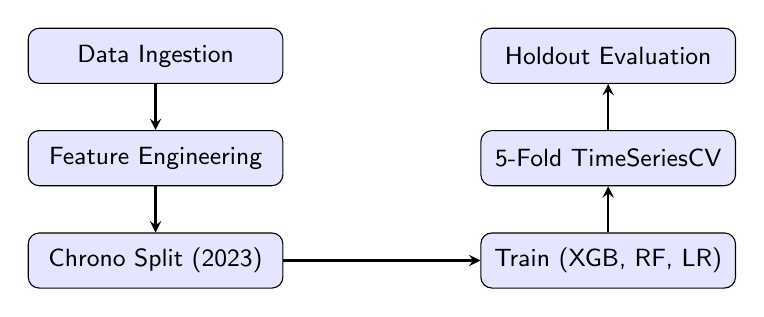
\begin{tikzpicture}[
            node distance=1.3cm,
            box/.style={rectangle, draw, fill=blue!10, text width=3cm, text centered, rounded corners, minimum height=0.7cm, font=\small},
            arrow/.style={->, >=stealth, thick}
        ]
            \node[box] (data) {Data Ingestion};
            \node[box, below of=data] (feat) {Feature Engineering};
            \node[box, below of=feat] (split) {Chrono Split (2023)};
            \node[box, right=2.5cm of split] (train) {Train (XGB, RF, LR)};
            \node[box, above of=train] (cv) {5-Fold TimeSeriesCV};
            \node[box, above of=cv] (eval) {Holdout Evaluation};

            \draw[arrow] (data) -- (feat);
            \draw[arrow] (feat) -- (split);
            \draw[arrow] (split) -- (train);
            \draw[arrow] (train) -- (cv);
            \draw[arrow] (cv) -- (eval);
        \end{tikzpicture}
    \end{center}

    \vspace{0.3cm}

    \begin{columns}
        \column{0.5\textwidth}
        \textbf{Train:} before 2023-01-01 (2,038 samples)\\
        \textbf{Test:} from 2023-01-01 (2,319 samples)

        \column{0.5\textwidth}
        \textbf{Scaling:} MinMaxScaler\\
        \textbf{CV metric:} Precision (5-fold)
    \end{columns}
\end{frame}

\begin{frame}{Model Comparison --- Results}
    \begin{table}
        \centering
        \begin{tabular}{lcccc}
            \toprule
            \textbf{Model} & \textbf{Accuracy} & \textbf{Precision} & \textbf{F1} & \textbf{ROC-AUC} \\
            \midrule
            XGBoost        & 53\% & 0.366 & 0.373 & 0.513 \\
            Random Forest  & 58\% & 0.390 & 0.303 & 0.518 \\
            Logistic Reg.  & 55\% & 0.399 & 0.406 & 0.506 \\
            \bottomrule
        \end{tabular}
    \end{table}

    \vspace{0.3cm}

    \begin{columns}
        \column{0.5\textwidth}
        \begin{center}
            \includegraphics[width=0.9\textwidth]{Confusion Matrix}
        \end{center}

        \column{0.5\textwidth}
        \textbf{Key Takeaways:}
        \begin{itemize}
            \item All models slightly above random (AUC $>$ 0.50)
            \item Logistic Regression competitive with tree models
            \item Stock prediction is inherently noisy --- these results are realistic
        \end{itemize}
    \end{columns}
\end{frame}

\begin{frame}{Threshold Tuning (from Notebook)}
    \textbf{Problem:} Default 0.5 may be suboptimal. We sweep thresholds and evaluate by \emph{Sharpe ratio} on the backtest.
    \vspace{0.25cm}
    \begin{columns}
        \column{0.5\textwidth}
        \begin{center}
            \includegraphics[width=\textwidth]{Precision_Recall_Coverage_vs_Threshold}
        \end{center}
        \column{0.45\textwidth}
        \textbf{From notebook:}
        \begin{itemize}
            \item Higher threshold $\Rightarrow$ fewer trades, often better precision
            \item Best threshold by Sharpe: \textbf{0.40}
            \item Trade-off: precision vs.\ coverage
        \end{itemize}
    \end{columns}
\end{frame}

\begin{frame}{Feature Importance (XGBoost)}
    \begin{center}
        \includegraphics[width=0.85\textwidth]{Top 15 Feature Importances (XGBoost)}
    \end{center}
    \vspace{0.2cm}
    \small Rolling-window stats (mean/std/last) of RSI, ATR, MACD, 10Y yield, etc.\ drive predictions; ablation in the notebook confirms which feature groups help.
\end{frame}

\begin{frame}{ROC \& Model Comparison}
    \begin{columns}
        \column{0.5\textwidth}
        \begin{center}
            \includegraphics[width=\textwidth]{ROC curve for the test set(xgboost)}
        \end{center}
        \column{0.5\textwidth}
        \begin{center}
            \includegraphics[width=\textwidth]{Model Comparison on Test Set}
        \end{center}
    \end{columns}
\end{frame}

\begin{frame}{Backtest \& Equity Curve}
    \begin{columns}
        \column{0.5\textwidth}
        \begin{center}
            \includegraphics[width=\textwidth]{Equity Curve (0.4)}
        \end{center}

        \column{0.5\textwidth}
        \textbf{Backtest Setup:}
        \begin{itemize}
            \item Non-overlapping 5-day windows
            \item Long-only / cash strategy
            \item Signal: BUY if $P(\text{up}) \geq$ \textbf{0.40} (best by Sharpe)
        \end{itemize}

        \vspace{0.3cm}

        \textbf{Metrics (threshold 0.4):}
        \begin{itemize}
            \item Annualized return, Sharpe, max drawdown from holdout
            \item Threshold chosen by risk-adjusted performance
        \end{itemize}
    \end{columns}
\end{frame}

% ============================================================
\section{Deployment --- Dashboard}
% ============================================================

\begin{frame}{Live Dashboard}
    % ---- PLACEHOLDER: insert full dashboard screenshot ----
    \begin{center}
        \fbox{\parbox{0.85\textwidth}{\centering\vspace{4.5cm}\textit{[Insert: Dashboard Screenshot]}\vspace{4.5cm}}}
    \end{center}
\end{frame}

% ============================================================
\section{Conclusion \& Future Work}
% ============================================================

\begin{frame}{Conclusion}
    \textbf{What we built:}
    \begin{enumerate}
        \item End-to-end ML pipeline: ingestion $\rightarrow$ features $\rightarrow$ training $\rightarrow$ evaluation $\rightarrow$ deployment
        \item Chronological train/test split (no data leakage)
        \item 3 models compared (XGBoost, Random Forest, Logistic Regression)
        \item Streamlit dashboard + FastAPI for serving predictions
    \end{enumerate}

    \vspace{0.3cm}

    \textbf{Lessons learned:}
    \begin{itemize}
        \item Stock prediction is hard --- 53\% accuracy is realistic for this domain
        \item More features $\neq$ better performance (we tested 40+ features, marginal gain)
        \item Temporal validation is critical to avoid overfitting
        \item Simple, interpretable pipelines are more valuable than complex ones
    \end{itemize}
\end{frame}

\begin{frame}{Future Work}
    \begin{columns}
        \column{0.5\textwidth}
        \textbf{Model Improvements:}
        \begin{itemize}
            \item Add sentiment features (FinBERT)
            \item Try deep learning (LSTM, Transformers)
            \item Ensemble stacking
            \item Probability calibration
        \end{itemize}

        \column{0.5\textwidth}
        \textbf{Engineering:}
        \begin{itemize}
            \item Dockerized deployment
            \item Automated retraining pipeline
            \item Model monitoring \& drift detection
            \item CI/CD for model updates
        \end{itemize}
    \end{columns}
\end{frame}

% ============================================================
% Thank You
% ============================================================

\begin{frame}[plain]
    \begin{center}
        \Huge \textbf{Thank You!}

        \vspace{1.5cm}

        \LARGE Questions?

        \vspace{1.5cm}

        \large
        \textbf{Dalil ADIMI \& Hassen BEN AMOR}\\
        Group I2-NEW DAI --- EFREI Paris
    \end{center}
\end{frame}

\end{document}
